\section*{BÀI TẬP CTLG - HSLG}
\setcounter{ex}{0}\setcounter{bt}{0}
\Opensolutionfile{ans}[ans/ans-OTB23]

\begin{ex}%[Dự án Toán 11-WTB-1]%[Cao Thành Thái]%[1K1Y2-2]
Khẳng định nào dưới đây \textbf{sai}?
\choice
{$2\sin^2 a=1-\cos 2a$}
{\True $\cos 2a=2\cos a-1$}
{$\sin 2a=2\sin a \cos a$}
{$\sin (a+b)=\sin a\cos b+\sin b\cos a$}
\loigiai
{
Công thức cộng $\sin (a+b)=\sin a\cos b+\sin b\cos a$.\\
Công thức nhân đôi $\sin 2a=2\sin a\cos a$, $\cos 2a=\cos^2 a-\sin^2 a= 2\cos^2 a-1 = 1-2\sin^2 a$.
}
\end{ex}

\begin{ex}%[Dự án Toán 11-WTB-1]%[Cao Thành Thái]%[1K1Y2-2]
Trong các công thức sau, công thức nào \textbf{sai}?
\choice
{$\cos 2a=\cos^2 a-\sin^2 a$}
{\True $\cos 2a=\cos^2 a+\sin^2 a$}
{$\cos 2a=2\cos^2 a-1$}
{$\cos 2a=1-2\sin^2 a$}
\loigiai
{
Ta có $\cos 2a=\cos^2 a-\sin^2 a= 2\cos^2 a-1 = 1-2\sin^2 a$.
}
\end{ex}

\begin{ex}%[Dự án Toán 11-WTB-1]%[Cao Thành Thái]%[1K1Y2-2]
Công thức nào dưới đây đúng?
\choice
{\True $\sin 2x=2\sin x \cos x$}
{$\sin 2x=\sin x \cos x$}
{$\sin 2x=2\cos x$}
{$\sin 2x=2\sin x$}
\loigiai
{
Công thức nhân đôi $\sin 2x=2\sin x\cos x$.
}
\end{ex}

\begin{ex}%[Dự án Toán 11-WTB-1]%[Cao Thành Thái]%[1K1Y2-3]
Với $\alpha$ là số thực bất kỳ, mệnh đề nào sau đây là mệnh đề đúng?
\choice
{$\cos 2\alpha+\cos 4\alpha=2\cos 2\alpha \cos 6\alpha$}
{$\sin 2\alpha+\sin 4\alpha=2\sin \alpha\cos 3\alpha$}
{$\cos 2\alpha-\cos 4\alpha=-2\sin 3\alpha\sin \alpha$}
{\True $\sin 2\alpha-\sin 4\alpha=-2\cos 3\alpha \sin \alpha$}
\loigiai
{
Ta có
\begin{itemize}
\item $\sin 2\alpha-\sin 4\alpha = 2\cos\left(\dfrac{2\alpha+4\alpha}{2}\right)\sin\left(\dfrac{2\alpha-4\alpha}{2}\right)=-2\cos 3\alpha \sin \alpha$.
\item $\sin 2\alpha+\sin 4\alpha = 2\sin\left(\dfrac{2\alpha+4\alpha}{2}\right)\cos\left(\dfrac{2\alpha-4\alpha}{2}\right)=2\sin 3\alpha \cos \alpha$.
\item $\cos 2\alpha+\cos 4\alpha = 2\cos\left(\dfrac{2\alpha+4\alpha}{2}\right)\cos\left(\dfrac{2\alpha-4\alpha}{2}\right)=2\cos 3\alpha \cos \alpha$.
\item $\cos 2\alpha-\cos 4\alpha = -2\sin\left(\dfrac{2\alpha+4\alpha}{2}\right)\sin\left(\dfrac{2\alpha-4\alpha}{2}\right)=2\sin 3\alpha \sin \alpha$.
\end{itemize}
}
\end{ex}

\begin{ex}%[1K1Y3-3]
Trong các khẳng định sau đây, khẳng định nào đúng?
\choice
{Hàm số $y=\sin x$ là hàm số chẵn}
{Hàm số $y=\cos x$ là hàm số lẻ}
{\True Hàm số $y=\tan x$ là hàm số lẻ}
{Hàm số $y=\cot x$ là hàm số chẵn}
\loigiai{
.
}
\end{ex}

\begin{ex}%[Dự án Toán 11-WTB-1]%[Lê Quốc Dũng]%[1K1Y2-3]
Trong các khẳng định sau, khẳng định nào \textbf{sai}?
\choice
{$\sin a-\sin b=2\cos \dfrac{a+b}{2}\sin \dfrac{a-b}{2}$}
{\True $\cos(a-b)=\cos a\cos b-\sin a\sin b$}
{$\sin(a-b)=\sin a\cos b-\cos a\sin b$}
{$2\cos a\cos b=\cos(a-b)+\cos(a+b)$}
\loigiai
{
Công thức cộng
\begin{itemize}
\item $\cos(a-b)=\cos a\cos b+\sin a\sin b$.
\item $\sin(a-b)=\sin a\cos b-\cos a\sin b$.
\end{itemize}
Công thức biến đổi tổng thành tích
\begin{itemize}
\item $\sin a-\sin b=2\cos \dfrac{a+b}{2}\sin \dfrac{a-b}{2}$.
\item $\cos(a-b)+\cos(a+b) = 2\cos\dfrac{a-b+a+b}{2}\cos\dfrac{a-b-a-b}{2} = 2\cos a\cos b$.
\end{itemize}
}
\end{ex}

\begin{ex}%[1K1Y3-5]
Giá trị lớn nhất của hàm số $y=3 \sin x$ trên tập xác định $\mathbb{R}$ là?
\choice
{$1$}
{$2$}
{\True $3$}
{$-3$}
\loigiai{
Hàm số $y=\sin x$ có tập giá trị là $[-1 ; 1]$. Do đó $-3 \leq 3 \sin x \leq 3, \forall x \in \mathbb{R}$.\\
Vậy giá trị lớn nhất của hàm số $y=3 \sin x$ trên tập xác định $\mathbb{R}$ là $3$, xảy ra khi $\sin x=1 \Leftrightarrow x=\dfrac{\pi}{2}+k 2 \pi$.
}
\end{ex}

\begin{ex}%[1K1Y3-5]
Giá trị nhỏ nhất của hàm số $y=\cos x$ là
\choice
{\True $1$}
{$0$}
{$-1$}
{$2$}
\loigiai{
Ta có $-1 \leq \cos x \leq 1, \forall x \in \mathbb{R}$ nên giá trị nhỏ nhất của hàm số $y=\cos x$ là $-1$ khi $x=\pi+k 2 \pi$.
}
\end{ex}

\begin{ex}%[Dự án Toán 11-WTB-1]%[Cao Thành Thái]%[1K1Y2-2]
Với $\alpha$ là số thực bất kỳ, trong các mệnh đề sau, mệnh đề nào \textbf{sai}?
\choice
{$\sin 2\alpha=2\sin \alpha \cos \alpha$}
{$\cos 2\alpha=2\cos^2 \alpha-1$}
{$\cos 2\alpha=-2\sin^2 \alpha+1$}
{\True $\cos 2\alpha=\sin^2 \alpha-\cos^2 \alpha$}
\loigiai
{
Ta có $\sin 2\alpha = 2\sin\alpha\cos\alpha$ và $\cos 2\alpha = \cos^2 \alpha-\sin^2 \alpha = 2\cos^2 \alpha-1 = 1-2\sin^2 \alpha$.
}
\end{ex}

\begin{ex}%[Dự án Toán 11-WTB-1]%[Cao Thành Thái]%[1K1Y2-2]
Biết $\cos (a-b)=\cos a \cos b+\sin a \sin b$. Với $a=-b$ thì $\cos 2a$ bằng
\choice
{$\cos^2 a+\sin^2 a$}
{$-\cos^2 a-\sin^2 a$}
{\True $\cos^2 a-\sin^2 a$}
{$\sin^2 a-\cos^2 a$}
\loigiai
{
Biết $\cos (a-b)=\cos a \cos b+\sin a \sin b$. Với $a=-b$ thì $\cos 2a = \cos^2 a-\sin^2 a$.
}
\end{ex}

\begin{ex}%[1K1Y3-1]
Tập xác định của hàm số $y=\tan 3x$ là.
\choice
{\True $\mathscr{D}=R \setminus \left\{ \dfrac{\pi}{6}+k\dfrac{\pi}{3},k \in \mathbb{R} \right\}$}
{$\mathscr{D}=R \setminus \left\{ \dfrac{\pi}{2}+k\pi,k \in \mathbb{R} \right\}$}
{$\mathscr{D}=R \setminus \left\{ \pi +k\pi,k \in \mathbb{R} \right\}$}
{$\mathscr{D}=R \setminus \left\{ k\dfrac{2\pi}{3},k \in \mathbb{R} \right\}$}
\loigiai{
Điều kiện $\cos 3x \ne 0 \Leftrightarrow 3x \ne \dfrac{\pi}{2}+k\pi \Leftrightarrow x \ne \dfrac{\pi}{6}+\dfrac{k\pi}{3}$.\\
Tập xác định: $\mathscr{D}=R \setminus \left\{ \dfrac{\pi}{6}+k\dfrac{\pi}{3},k \in \mathbb{R} \right\}$.
}
\end{ex}


\begin{ex}%[Dự án Toán 11-WTB-1]%[Lê Quốc Dũng]%[1K1B2-1]
Cho $\sin \alpha =\dfrac{3}{5}$, $\left(\dfrac{\pi}{2}<\alpha <\pi\right)$. Giá trị của $\tan \left(\alpha +\dfrac{\pi}{3} \right)$ bằng
\choice
{$\dfrac{48+25\sqrt{3}}{11}$}
{$\dfrac{8-5\sqrt{3}}{11}$}
{$\dfrac{8-\sqrt{3}}{11}$ }
{\True  $\dfrac{48-25 \sqrt{3}}{11}$}
\loigiai
{
Ta có
\[\cos^2 \alpha = 1-\sin^2 \alpha \Leftrightarrow \cos^2 \alpha = 1-\left(\dfrac{3}{5}\right)^2 \Leftrightarrow \cos^2 \alpha = \dfrac{16}{25} \Leftrightarrow \cos \alpha=\pm\dfrac{4}{5}.\]
Vì $\dfrac{\pi}{2}<\alpha <\pi$ nên $\cos \alpha<0$. Do đó, $\cos \alpha=-\dfrac{4}{5}$.\\
Khi đó $\tan\alpha = \dfrac{\sin\alpha}{\cos\alpha} = \dfrac{\dfrac{3}{5}}{-\dfrac{4}{5}} = -\dfrac{3}{4}$.\\
Vậy $\tan \left(\alpha+\dfrac{\pi}{3}\right) =\dfrac{\tan \alpha+\tan \dfrac{\pi}{3}}{1-\tan \alpha \tan \dfrac{\pi}{3}}=\dfrac{-\dfrac{3}{4}+\sqrt{3}}{1-\left(-\dfrac{3}{4}\right)\cdot \sqrt{3}} = \dfrac{48-25 \sqrt{3}}{11}$.
}
\end{ex}

\begin{ex}%[Dự án Toán 11-WTB-1]%[Lê Quốc Dũng]%[1K1B2-1]
Rút gọn biểu thức $\cos \left(120^\circ- x\right)+\cos \left(120^\circ +x\right)-\cos x$ ta được kết quả là
\choice
{$0$}
{$-\cos x$}
{\True $-2\cos x$}
{$\sin x-\cos x$}
\loigiai
{
Ta có $\cos \left(120^\circ -x\right)+\cos \left(120^\circ +x\right)-\cos x =-\dfrac{1}{2}\cos x+\dfrac{\sqrt{3}}{2}\sin x-\dfrac{1}{2}\cos x - \dfrac{\sqrt{3}}{2}\sin x-\cos x =-2\cos x$.
}
\end{ex}

\begin{ex}%[Dự án Toán 11-WTB-1]%[Cao Thành Thái]%[1K1B2-2]
Nếu $\sin x+\cos x=\dfrac{1}{2}$ thì $\sin 2x$ bằng
\choice
{$\dfrac{3}{4}$}
{$\dfrac{3}{8}$}
{$\dfrac{\sqrt{2}}{2}$}
{\True $-\dfrac{3}{4}$}
\loigiai
{
Từ $\sin x+\cos x=\dfrac{1}{2}$ suy ra
\[(\sin x+\cos x)^2=\left(\dfrac{1}{2}\right)^2 \Leftrightarrow \sin^2 x+2\sin x\cos x+\cos^2 x=\dfrac{1}{4} \Leftrightarrow \sin 2x+1=\dfrac{1}{4} \Leftrightarrow \sin 2x=-\dfrac{3}{4}.\]
}
\end{ex}

\begin{ex}%[Dự án Toán 11-WTB-1]%[Lê Quốc Dũng]%[1K1B2-1]
Biết $\sin a=\dfrac{5}{13}$, $\cos b=\dfrac{3}{5}$, $\left(\dfrac{\pi}{2}<a<\pi,\,0<b<\dfrac{\pi}{2}\right)$. Giá trị của $\sin(a+b)$ bằng
\choice
{\True $\dfrac{-33}{65}$}
{$\dfrac{63}{65}$}
{$\dfrac{56}{65}$}
{$0$}
\loigiai
{
Ta có
\[\cos^2 a = 1-\sin^2 a \Leftrightarrow \cos^2 a = 1-\left(\dfrac{5}{13}\right)^2 \Leftrightarrow \cos^2 a = \dfrac{144}{169} \Leftrightarrow \cos a = \pm\dfrac{12}{13}.\]
Vì $\dfrac{\pi}{2}<a<\pi$ nên $\cos a<0$. Do đó, $\cos \alpha=-\dfrac{12}{13}$.\\
Ta có
\[\sin^2 b = 1-\cos^2 b \Leftrightarrow \sin^2 b = 1-\left(\dfrac{3}{5}\right)^2 \Leftrightarrow \sin^2 b = \dfrac{16}{25} \Leftrightarrow \sin b = \pm\dfrac{4}{5}.\]
Vì $0<b<\dfrac{\pi}{2}$ nên $\sin b>0$. Do đó, $\sin b=\dfrac{4}{5}$.\\
Vậy $\sin (a+b)=\sin a\cos b+\cos a\sin b=\dfrac{5}{13}\cdot \dfrac{3}{5}+\dfrac{-12}{13}\cdot \dfrac{4}{5}=-\dfrac{33}{65}$.
}
\end{ex}

\begin{ex}%[1K1B3-1]
Hàm số $y=\dfrac{\sin 2x}{\cot x-\sqrt{3}}$ có tập xác định là
\choice
{$\mathscr{D}=\mathbb{R} \setminus \left\{ \dfrac{\pi}{6}+k\pi |k \in \mathbb{Z} \right\}$}
{$\mathscr{D}=\mathbb{R} \setminus \left\{ k\pi |k \in \mathbb{Z} \right\}$}
{\True $\mathscr{D}=\mathbb{R} \setminus \left\{ k\pi;\dfrac{\pi}{6}+k\pi |k \in \mathbb{Z} \right\}$}
{$\mathscr{D}=\mathbb{R} \setminus \left\{ \dfrac{\pi}{2}+k\pi;\dfrac{\pi}{6}+k\pi |k \in \mathbb{Z} \right\}$}
\loigiai{
Điều kiện xác định của hàm số là: $\heva{&\cot x \ne \sqrt{3}\\&\sin x \ne 0} \Leftrightarrow \heva{&x \ne \dfrac{\pi}{6}+k\pi \\&x \ne k\pi}\left( k \in \mathbb{Z} \right)$.
}
\end{ex}

\begin{ex}%[Thành Đức Trung, Hàm số - Đợt 2 - Tư duy mở]%[1K1B3-5]
Giá trị nhỏ nhất của hàm số $f(x)=2\cos x + 2 \sin\left(x-\dfrac{\pi}{3}\right)$ bằng
\choice
{\True $-\sqrt{8-4\sqrt{3}}$}
{$2\sqrt{2}$}
{$4$}
{$-2\sqrt{2}$}
\loigiai
{Ta có $f(x)=2\cos x +2 \left(\sin x\cdot\cos \dfrac{\pi}{3}-\cos x \cdot \sin \dfrac{\pi}{3}\right)=\left(2-\sqrt{3}\right)\cos x+\sin x$. \\
Tập xác định $\mathscr{D} =\mathbb{R}$.\\
Với mọi $x\in \mathbb{R}$, ta có $\left(2-\sqrt{3}\right)\cos x+\sin x \geq-\sqrt{\left(2-\sqrt{3}\right)^2+1^2}=-\sqrt{8-4\sqrt{3}}$. \\
Vậy $\min\limits_{\mathbb{R}} f(x) = -\sqrt{8-4\sqrt{3}}$.
}
\end{ex}

\begin{ex}%[Dự án Toán 11-WTB-1]%[Lê Quốc Dũng]%[1K1B2-1]
Cho $\sin x=\dfrac{3}{5}$, với $\dfrac{\pi }{2}<x<\pi$, khi đó $\tan \left(x+\dfrac{\pi}{4}\right)$ bằng
\choice
{$\dfrac{2}{7}$}
{$-\dfrac{1}{7}$}
{$-\dfrac{2}{7}$}
{\True $\dfrac{1}{7}$}
\loigiai
{
Ta có
\[\cos^2 x = 1-\sin^2 x \Leftrightarrow \cos^2 x = 1-\left(\dfrac{3}{5}\right)^2 \Leftrightarrow \cos^2 x = \dfrac{16}{25} \Leftrightarrow \cos x=\pm\dfrac{4}{5}.\]
Vì $\dfrac{\pi}{2}<x<\pi$ nên $\cos x<0$. Do đó, $\cos x=-\dfrac{4}{5}$.\\
Khi đó $\tan x = \dfrac{\sin x}{\cos x} = \dfrac{\dfrac{3}{5}}{-\dfrac{4}{5}} = -\dfrac{3}{4}$.\\
Vậy $\tan \left(x+\dfrac{\pi}{4}\right) = \dfrac{\tan x+\tan \dfrac{\pi}{4}}{1-\tan x\tan \dfrac{\pi}{4}}=\dfrac{-\dfrac{3}{4}+1}{1+\dfrac{3}{4}\cdot 1}=\dfrac{1}{7}$.
}
\end{ex}

\begin{ex}%[1K1B3-1]
Hàm số $y=\dfrac{\tan x}{1+\tan x}$ không xác định tại các điểm
\choice
{chỉ $x=\dfrac{\pi}{2}+k\pi$ $\left( k \in \mathbb{Z} \right)$}
{chỉ $x=\dfrac{\pi}{4}+k\pi$ $\left( k \in \mathbb{Z} \right)$}
{chỉ $x=-\dfrac{\pi}{4}+k\pi$ $\left( k \in \mathbb{Z} \right)$}
{\True $x=-\dfrac{\pi}{4}+k\pi$ và $x=\dfrac{\pi}{2}+k\pi$ $\left( k \in \mathbb{Z} \right)$}
\loigiai{
Hàm số không xác định khi $\hoac{&1+\tan x=0\\&\cos x=0} \Leftrightarrow \hoac{&x=-\dfrac{\pi}{4}+k\pi \\&x=\dfrac{\pi}{2}+k\pi}\left( k \in \mathbb{Z} \right)$.
}
\end{ex}

\begin{ex}%[Dự án Toán 11 -WTB-1]%[Hiếu Phan]%[1K1B3-1]
Tìm tập xác định của hàm số $y=2021\cot 2x+2022$.
\choice
{$\mathscr{D}=\mathbb{R}\setminus\left\{\dfrac{\pi}{2}+k\pi\right\}$}
{\True $\mathscr{D}=\mathbb{R}\setminus\left\{ k\dfrac{\pi}{2}\right\}$}
{$\mathscr{D}=\mathbb{R}\setminus\left\{\dfrac{\pi}{4}+k\dfrac{\pi}{2}\right\}$}
{$\mathscr{D}=\mathbb{R}$}
\loigiai{
Điều kiện xác định $\sin 2x\ne 0\Leftrightarrow 2x\ne k\pi\Leftrightarrow x\ne\dfrac{k\pi}{2},k\in\mathbb{Z}$.\\
Tập xác định $\mathscr{D}=\mathbb{R}\setminus\left\{ k\dfrac{\pi}{2};k\in\mathbb{Z}\right\}$.}
\end{ex}

\begin{ex}%[1K1B3-1]
Tập xác định của hàm số $y=\dfrac{1}{\tan x}$ là
\choice
{$\mathscr{D}=\left\{ k\dfrac{\pi}{2},k \in \mathbb{Z} \right\}$}
{\True $\mathscr{D}=\mathbb{R} \setminus \left\{ k\dfrac{\pi}{2},k \in \mathbb{Z} \right\}$}
{$\mathscr{D}=\mathbb{R} \setminus \left\{ k\pi,k \in \mathbb{Z} \right\}$}
{$\mathscr{D}=\left\{ k\pi,k \in \mathbb{Z} \right\}$}
\loigiai{
Điều kiện xác định: $\heva{&\cos x \ne 0\\&\tan x \ne 0}$ $\Leftrightarrow \heva{&\cos x \ne 0\\&\sin x \ne 0}$ $\Leftrightarrow \sin 2x \ne 0$ $\Leftrightarrow 2x \ne k\pi$ $\Leftrightarrow x \ne k\dfrac{\pi}{2},k \in \mathbb{Z}$.\\
Vậy tập xác định của hàm số đã cho là $\mathscr{D}=\mathbb{R} \setminus \left\{ k\dfrac{\pi}{2},k \in \mathbb{Z} \right\}$.
}
\end{ex}

\begin{ex}%[1K1B3-5]
Tập giá trị của hàm số $y=\sin 4 x-3$ là
\choice
{\True $[-4;-2]$}
{$[-3;1]$}
{$[-2;2]$}
{$[-4;2]$}
\loigiai{
Do $-1 \leq \sin 4 x \leq 1, \forall x \in \mathbb{R}$ nên $-4 \leq \sin 4 x-3 \leq-2, \forall x \in \mathbb{R}$.\\
Vậy tập giá trị của hàm số là $[-4 ;-2]$.

}
\end{ex}

\begin{ex}%[Dự án Toán 11-WTB-1]%[Cao Thành Thái]%[1K1B2-2]
Cho $\sin 2\alpha=\dfrac{3}{4}$. Giá trị biểu thức $A=\tan \alpha+\cot \alpha$ là
\choice
{$A=\dfrac{4}{3}$}
{$A=\dfrac{2}{3}$}
{\True $A=\dfrac{8}{3}$}
{$A=\dfrac{16}{3}$}
\loigiai
{
Ta có $A=\tan \alpha+\cot \alpha=\dfrac{\sin \alpha}{\cos \alpha}+\dfrac{\cos \alpha}{\sin \alpha}=\dfrac{\sin ^2 \alpha+\cos ^2 \alpha}{\sin \alpha \cos \alpha}=\dfrac{1}{\dfrac{1}{2} \sin 2\alpha}=\dfrac{1}{\dfrac{1}{2} \cdot \dfrac{3}{4}}=\dfrac{8}{3}$.
}
\end{ex}

\begin{ex}%[1K1B3-1]
Tập xác định của hàm số $y=\dfrac{3\cot x}{2\sin x-4}$ là
\choice
{$\mathbb{R} \setminus \left\{ \arcsin 2+k2\pi,\pi -\arcsin 2+k2\pi,k \in \mathbb{Z} \right\}$}
{$\mathbb{R}$}
{$\mathbb{R} \setminus \left\{ \pm \arcsin 2+k2\pi,k \in \mathbb{Z} \right\}$}
{\True $\mathbb{R} \setminus \left\{ k\pi,k \in \mathbb{Z} \right\}$}
\loigiai{
Ta có $2\sin x-4 \ne 0,\,\forall x \in \mathbb{R}$,\\
Nên hàm số xác định khi $\cot x$ xác định $\Leftrightarrow$ $\sin x \ne 0 \Leftrightarrow x \ne k\pi,k \in \mathbb{Z}$\\
Vậy tập xác định của hàm số là $R \setminus \left\{ k\pi,k \in \mathbb{Z} \right\}$.
}
\end{ex}

\begin{ex}%[Dự án Toán 11-WTB-1]%[Cao Thành Thái]%[1K1B2-4]
Cho biết $\cos \alpha=-\dfrac{2}{3}$. Giá trị của biểu thức $P=\dfrac{\cot \alpha+3\tan \alpha}{2\cot \alpha+\tan \alpha}$ bằng bao nhiêu?
\choice
{\True $P=\dfrac{19}{13}$}
{$P=\dfrac{25}{13}$}
{$P=-\dfrac{25}{13}$}
{$P=-\dfrac{19}{13}$}
\loigiai
{
Ta có $\tan^2 \alpha = \dfrac{1}{\cos^2\alpha}-1 = \dfrac{1}{\dfrac{4}{9}}-1 = \dfrac{5}{4}$. Suy ra $\tan x\neq 0$.\\
Khi đó
\[P=\dfrac{\cot \alpha+3\tan \alpha}{2\cot \alpha+\tan \alpha} = \dfrac{\dfrac{1}{\tan\alpha} + 3\tan\alpha}{\dfrac{2}{\tan\alpha} + \tan\alpha} = \dfrac{1+3\tan^2 \alpha}{2+\tan^2 \alpha} = \dfrac{1+3\cdot \dfrac{5}{4}}{2+\dfrac{5}{4}} = \dfrac{19}{13}.\]
}
\end{ex}

\begin{ex}%[1K1B3-5]
Giá trị lớn nhất và giá trị nhỏ nhất của hàm số $y=3 \sin \left(x+\dfrac{3 \pi}{4}\right)-1$ lần lượt là
\choice
{$4$; $-2$}
{\True $2$; $-4$}
{$1$; $-1$}
{$3$; $-3$}
\loigiai{
Tập xác định $\mathscr{D}=\mathbb{R}$.\\
$\forall x \in \mathbb{R}$ ta có\\
\[-1 \leq \sin \left(x+\dfrac{3 \pi}{4}\right) \leq 1 \Leftrightarrow-3 \leq 3 \sin \left(x+\dfrac{3 \pi}{4}\right) \leq 3 \Leftrightarrow-4 \leq 3 \sin \left(x+\dfrac{3 \pi}{4}\right)-1 \leq 2\Rightarrow-4 \leq y \leq 2.\]
Vậy giá trị lớn nhất của hàm số $y=3 \sin \left(x+\dfrac{3 \pi}{4}\right)-1$ là $2$ khi $x=-\dfrac{\pi}{4}$.\\
Giá trị nhỏ nhất của hàm số $y=3 \sin \left(x+\dfrac{3 \pi}{4}\right)-1$ là $-4$ khi $x=\dfrac{3 \pi}{4}$.
}
\end{ex}

\begin{ex}%[Dự án Toán 11 -WTB-1]%[Hiếu Phan]%[1K1B3-1]
Tập xác định của hàm số $y=2+3\tan x$ là
\choice
{$\mathscr{D}=\mathbb{R}\setminus\left\{\dfrac{\pi}{3}+k\pi\right\}$}
{$\mathscr{D}=\mathbb{R}\setminus\left\{\dfrac{\pi}{6}+k\pi\right\}$}
{\True $\mathscr{D}=\mathbb{R}\setminus\left\{\dfrac{\pi}{2}+k\pi\right\}$}
{$\mathscr{D}=\mathbb{R}\setminus\left\{\dfrac{\pi}{4}+k\pi\right\}$}
\loigiai{
Điều kiện xác định $\cos x\ne 0\Leftrightarrow x\ne\dfrac{\pi}{2}+k\pi $.\\
Do đó tập xác định của hàm số là $\mathscr{D}=\mathbb{R}\setminus\left\{\dfrac{\pi}{2}+k\pi\right\}$.}
\end{ex}

\begin{ex}%[1K1B3-5]
Tìm giá trị lớn nhất và giá trị nhỏ nhất của hàm số $y=8 \sin 2 x-5$.
\choice
{$\max y=11$; $\min y=-21$}
{$\max y=8$; $\min y=-8$}
{$\max y=-4$; $\min y=-6$}
{\True $\max y=3$; $\min y=-13$}
\loigiai{
Ta có $-1 \leq \sin 2 x \leq 1 \Leftrightarrow-8 \leq 8 \sin 2 x \leq 8 \Leftrightarrow-13 \leq 8 \sin 2 x-5 \leq 3$.\\
Vậy giá trị lớn nhất của hàm số đã cho là $3$ khi $\sin2x=1\Leftrightarrow x=\dfrac{\pi}{4}+k\pi$.\\
Giá trị nhỏ nhất của hàm số đã cho là $-13$ khi $\sin2x=-1\Leftrightarrow x=-\dfrac{\pi}{4}+k\pi$.
}
\end{ex}

\begin{ex}%[Dự án Toán 11-WTB-1]%[Lê Quốc Dũng]%[1K1B2-1]
Biểu thức $A=\cos^2x+\cos^2\left(\dfrac{\pi }{3}+x \right)+\cos^2\left(\dfrac{\pi }{3}-x \right)$ không phụ thuộc $x$ và bằng
\choice
{$\dfrac{3}{4}$}
{$\dfrac{4}{3}$}
{\True $\dfrac{3}{2}$}
{$\dfrac{2}{3}$}
\loigiai
{
Ta có
\allowdisplaybreaks
\begin{eqnarray*}
A &=& \cos^2 x+\cos^2\left(\dfrac{\pi}{3}+x\right)+\cos^2 \left(\dfrac{\pi}{3}-x\right) =\cos^2x+\left( \dfrac{1}{2}\cos x-\dfrac{\sqrt{3}}{2}\sin x \right)^2+\left( \dfrac{1}{2}\cos x+\dfrac{\sqrt{3}}{2}\sin x \right)^2\\
&=& \cos^2 x+\dfrac{1}{4}\cos^2 x-\dfrac{\sqrt{3}}{2}\sin x\cos  x+\dfrac{3}{4}\sin^2 x+\dfrac{1}{4}\cos^2 x+\dfrac{\sqrt{3}}{2}\sin x\cos x+\dfrac{3}{4}\sin^2 x\\
&=& \dfrac{3}{2}\sin^2 x+\dfrac{3}{2}\cos^2 x = \dfrac{3}{2}\left(\sin^2 x+\cos^2 x\right) = \dfrac{3}{2}.
\end{eqnarray*}
}
\end{ex}

\begin{ex}%[Dự án Toán 11 -WTB-1]%[Hiếu Phan]%[1K1B3-1]
Tập xác định của hàm số $y=\dfrac{2\sin x+1}{1-\cos x}$ là
\choice
{\True $\mathscr{D}=\mathbb{R}\setminus\left\{ x\ne k2\pi ;k\in\mathbb{Z}\right\}$}
{$\mathscr{D}=\mathbb{R}\setminus\left\{ x\ne\pi+k2\pi ;k\in\mathbb{Z}\right\}$}
{$\mathscr{D}=\mathbb{R}\setminus\left\{ x\ne\dfrac{\pi}{2}+k\pi ;k\in\mathbb{Z}\right\}$}
{$\mathscr{D}=\mathbb{R}\setminus\left\{ x\ne\dfrac{\pi}{2}+k2\pi ;k\in\mathbb{Z}\right\}$}
\loigiai{
Hàm số xác định khi $1-\cos x\ne 0\Leftrightarrow\cos x\ne 1\Leftrightarrow x\ne k2\pi $ , $k\in\mathbb{Z}$.}
\end{ex}


\begin{ex}%[Dự án Toán 11-WTB-1]%[Cao Thành Thái]%[1K1K2-4]
Tổng $A=\tan 9^\circ+\cot 9^\circ+\tan 15^\circ+\cot 15^\circ - \tan 27^\circ - \cot 27^\circ$ bằng
\choice
{$4$}
{$-4$}
{\True $8$}
{$-8$}
\loigiai
{
Ta có
\allowdisplaybreaks
\begin{eqnarray*}
A &=& \tan 9^\circ+\cot 9^\circ+\tan 15^\circ+\cot 15^\circ - \tan 27^\circ - \cot 27^\circ = \dfrac{\sin 9^\circ}{\cos 9^\circ} + \dfrac{\cos 9^\circ}{\sin 9^\circ}  + \dfrac{\sin 15^\circ}{\cos 15^\circ} + \dfrac{\cos 15^\circ}{\sin 15^\circ} - \left(\dfrac{\sin 27^\circ}{\cos 27^\circ} + \dfrac{\cos 27^\circ}{\sin 27^\circ} \right)\\
&=& \dfrac{\sin^2 9^\circ + \cos^2 9^\circ}{\sin 9^\circ\cos 9^\circ} + \dfrac{\sin^2 15^\circ + \cos^2 15^\circ}{\sin 15^\circ\cos 15^\circ} - \left(\dfrac{\sin^2 27^\circ + \cos^2 27^\circ}{\sin 27^\circ\cos 27^\circ}\right) = \dfrac{2}{\sin 18^\circ} + \dfrac{2}{\sin 30^\circ} - \dfrac{2}{\sin 54^\circ}\\
&=& 2\left(\dfrac{1}{\sin 18^\circ} - \dfrac{1}{\sin 54^\circ}\right) + 4 = 2\cdot \dfrac{\sin 54^\circ - \sin 18^\circ}{\sin 18^\circ\sin 54^\circ} + 4 = 2\cdot \dfrac{2\cos 36^\circ \sin 18^\circ}{\sin 18^\circ \sin \left(90^\circ - 36^\circ\right)} + 4 = \dfrac{4\cos 36^\circ}{\cos 36^\circ} + 4\\
&=& 4+4=8.
\end{eqnarray*}
}
\end{ex}

\begin{ex}%[Dự án Toán 11-WTB-1]%[Cao Thành Thái]%[1K1K2-3]
Rút gọn biểu thức $A=\dfrac{\sin x+\sin 2x+\sin 3x}{\cos x+\cos 2x+\cos 3x}$ ($\cos 2x\neq 0$, $2\cos x+1\neq 0$) ta được kết quả là
\choice
{$A=\tan 6x$}
{$A=\tan 3x$}
{\True $A=\tan 2x$}
{$A=\tan x+\tan 2x+\tan 3x$}
\loigiai
{
Với mọi $x$ thỏa mãn $\cos 2x\neq 0$, $2\cos x+1\neq 0$, ta có
\[A=\dfrac{\sin x+\sin 2x+\sin 3x}{\cos x+\cos 2x+\cos 3x} = \dfrac{(\sin 3x+\sin x)+\sin 2x}{(\cos 3x+\cos x)+\cos 2x}=\dfrac{2\sin 2x \cos x+\sin 2x}{2\cos 2x \cos x+\cos 2x}=\dfrac{\sin 2x(2\cos x+1)}{\cos 2x(2\cos x+1)}=\tan 2x.\]
}
\end{ex}

\begin{ex}%[Dự án Toán 11-WTB-1]%[Cao Thành Thái]%[1K1K2-3]
Biết $\cos a=\dfrac{1}{3}$, $\cos b=\dfrac{1}{4}$. Giá trị của biểu thức $\cos (a+b) \cos (a-b)$ bằng
\choice
{\True $-\dfrac{119}{144}$}
{$-\dfrac{115}{144}$}
{$-\dfrac{113}{144}$}
{$-\dfrac{117}{144}$}
\loigiai
{
Ta có $\cos (a+b) \cos (a-b)=\dfrac{1}{2}\left[\cos(a+b+a-b)+\cos(a+b-a+b)\right]=\dfrac{1}{2}(\cos 2a+\cos 2b)$.\\
Lại có $\cos 2a=2\cos^2 a-1 = 2\cdot \left(\dfrac{1}{3}\right)^2-1 = -\dfrac{7}{9}$ và $\cos 2b=2\cos^2 b-1 = 2\cdot \left(\dfrac{1}{4}\right)^2-1 = -\dfrac{7}{8}$.\\
Vậy $\cos (a+b) \cos (a-b) = \dfrac{1}{2}\cdot\left(-\dfrac{7}{9}-\dfrac{7}{8}\right) = -\dfrac{119}{144}$.
}
\end{ex}

\begin{ex}%[Dự án Toán 11-WTB-1]%[Lê Quốc Dũng]%[1K1K2-1]
Biết $\alpha +\beta +\gamma =\dfrac{\pi}{2}$ và $\cot \alpha$, $\cot \beta$, $\cot \gamma $ theo thứ tự lập thành một cấp số cộng. Tích số $\cot \alpha\cot \gamma$ bằng
\choice
{$2$}
{$-2$}
{\True $3$}
{$-3$}
\loigiai
{
Vì $\cot \alpha$, $\cot \beta$, $\cot \gamma $ theo thứ tự lập thành một cấp số cộng nên $\cot \alpha + \cot \gamma = 2\cot \beta$.\\
Từ $\alpha +\beta +\gamma =\dfrac{\pi }{2}$ ta có
\[\cot \beta = \cot\left[\dfrac{\pi}{2}-(\alpha+\gamma)\right] =\tan \left(\alpha +\gamma\right)=\dfrac{\tan \alpha +\tan \gamma}{1-\tan \alpha \tan \gamma} = \dfrac{\dfrac{1}{\cot \alpha} + \dfrac{1}{\cot \gamma}}{1-\dfrac{1}{\cot \alpha}\cdot \dfrac{1}{\cot \gamma}} =\dfrac{\cot \alpha +\cot\gamma }{\cot \alpha \cot\gamma -1}=\dfrac{2\cot \beta }{\cot \alpha \cot \gamma -1}.\]
Từ trên suy ra
\[\cot \beta = \dfrac{2\cot \beta}{\cot \alpha\cot \gamma-1} \Leftrightarrow 1=\dfrac{2}{\cot \alpha\cot \gamma-1} \Leftrightarrow \cot \alpha \cot \gamma -1 = 2 \Leftrightarrow \cot \alpha \cot \gamma =3.\]
Vậy $\cot \alpha \cot \gamma =3$.
}
\end{ex}

\begin{ex}%[Dự án Toán 11-WTB-1]%[Lê Minh Thiện Anh]%[1K1K3-5]
Giá trị lớn nhất của $M=\sin^6 x-\cos^6 x$ bằng
\choice
{$2$}
{$3$}
{$0$}
{\True $1$}
\loigiai
{
Ta có
\allowdisplaybreaks
\begin{eqnarray*}
M&= & \sin^6 x-\cos^6 x = \left(\sin^2 x-\cos^2 x\right)\left(\sin^4 x+\sin^2 x\cos^2 x+\cos^4 x\right) = -\cos 2x\left[\left(\sin^2 x+\cos^2 x\right)^2-\sin^2 x\cos^2 x\right]\\
&= & -\cos 2x\left(1-\dfrac{1}{4}\sin^2 2x\right) = -\cos 2x\left(\dfrac{3}{4}+\dfrac{1}{4} \cos^2 2x\right)\\
&\leq & \dfrac{3}{4}+\dfrac{1}{4}{\cos^{2}}2x\le \dfrac{3}{4}+\dfrac{1}{4}=1 \,\left(\text{do }\cos 2x\le 1 \right).
\end{eqnarray*}
Dấu ``$=$'' xảy ra khi và chỉ khi
\[\cos 2x=-1 \Leftrightarrow 2x=\pi+k2\pi, k\in\mathbb{Z} \Leftrightarrow x=\dfrac{\pi}{2}+k\pi, k\in\mathbb{Z}.\]
Vậy giá trị lớn nhất của $M$ là $1$.
}
\end{ex}

\begin{ex}%[1K1K3-1]
Hàm số $y=\dfrac{3+\sin 2x}{\sqrt{m\cos x+1}}$ có tập xác định là $\mathbb{R}$ khi
\choice
{$m>0$}
{$0 \leq m<1$}
{\True $-1<m<1$}
{$m \ne -1$}
\loigiai{
Hàm số $y=\dfrac{3+\sin 2x}{\sqrt{m\cos x+1}}$ có tập xác định là $\mathbb{R}$ $\Leftrightarrow m\cos x+1>0, \forall x\in \mathbb{R}$.
\begin{itemize}
\item $m=0 \Rightarrow 1>0\forall x \in \mathbb{R} \Rightarrow m=0$ thỏa ycbt.
\item  $m>0$\\
Ta có $-1 \leq \cos x \leq 1 \Rightarrow$ $-m \leq m\cos x \leq m \Rightarrow -m+1<m\cos x+1<m+1$\\
$\Rightarrow$ GTNN của $m\cos x+1$ là $-m+1$\\
$\Rightarrow -m+1>0 \Rightarrow 0<m<1$.
\item $m<0$\\
Ta có $-1 \leq \cos x \leq 1 \Rightarrow$ $-m \geq m\cos x \geq m \Rightarrow -m+1 \geq m\cos x+1 \geq m+1$\\
$\Rightarrow$ GTNN của $m\cos x+1$ là $m+1$\\
$\Rightarrow m+1>0 \Rightarrow -1<m<0$.
\end{itemize}
Suy ra: $-1<m<1$.
}
\end{ex}

\begin{ex}%[Dự án Toán 11-WTB-1]%[Lê Minh Thiện Anh]%[1K1K2-5]
Cho $A$, $B$, $C$ là ba góc của một tam giác. Đẳng thức nào dưới đây \textbf{sai}?
\choice
{$\cos \dfrac{A+B}{2}=\sin \dfrac{C}{2}$}
{$\cos (A+B+2C)=-\cos C$}
{\True $\sin (A+C)=-\sin B$}
{$\cos (A+B)=-\cos C$}
\loigiai
{
Với $A$, $B$, $C$ là các góc của tam giác $ABC$, ta có
\begin{itemize}
\item $\sin (A+C)=\sin(A+B+C-B) = \sin\left(180^\circ-B\right) = \sin B$.
\item $\cos (A+B)=\cos(A+B+C-C) = \cos\left(180^\circ-C\right) = -\cos C$.
\item $\cos (A+B+2C) = \cos\left(180^\circ+C\right)=-\cos C$.
\item $\cos \dfrac{A+B}{2} = \cos\left(\dfrac{A+B+C-C}{2}\right) = \cos\left(90^\circ-\dfrac{C}{2}\right)=\sin \dfrac{C}{2}$.
\end{itemize}
}
\end{ex}

\begin{ex}%[1K1K3-5]
Tìm giá trị lớn nhất của hàm số $y=\sin ^2 x-\cos x+2$.
\choice
{$3$}
{\True $\dfrac{13}{4}$}
{$\dfrac{7}{4}$}
{$1$}
\loigiai{
Ta có: $y=\sin ^2 x-\cos x+2=-\cos ^2 x-\cos x+3$.\\
Đặt $t=\cos x, t \in[-1 ; 1]$. Khi đó $y=f(t)=-t^2-t+3$.\\
Bảng biến thiên hàm số $f(t)$ trên $[-1 ; 1]$
\begin{center}
\begin{tikzpicture}
\tkzTabInit[nocadre=false,lgt=1.2,espcl=2.5,deltacl=0.6]
{$t$ /1.2,$f(t)$ /2}
{$-1$,$-\dfrac{1}{2}$,$1$}
\tkzTabVar{-/$3$, +/$\dfrac{13}{4}$,-/$1$}
\end{tikzpicture}
\end{center}
Vậy giá trị lớn nhất của hàm số đã cho là $\dfrac{13}{4}$ khi $\cos x=-\dfrac{1}{2} \Leftrightarrow x= \pm \dfrac{2 \pi}{3}+k 2 \pi$.
}
\end{ex}

\begin{ex}%[Dự án Toán 11-WTB-1]%[Cao Thành Thái]%[1K1K3-5]
Giá trị nhỏ nhất của $\sin^6 x+\cos^6 x$ là
\choice
{$0$}
{$\dfrac{1}{2}$}
{\True $\dfrac{1}{4}$}
{$\dfrac{1}{8}$}
\loigiai
{
Ta có
\[\sin^6 x+\cos^6 x=\left(\sin^2 x+\cos^2 x\right)^3-3\sin^2 x \cos^2 x\left(\sin^2 x+\cos^2 x\right)=1-\dfrac{3}{4} \sin^2 2x \geq 1-\dfrac{3}{4}=\dfrac{1}{4}.\]
Dấu ``$=$'' xảy ra khi và chỉ khi
\[\sin ^2 2x=1\Leftrightarrow \cos 2x=0 \Leftrightarrow 2x=\dfrac{\pi}{2}+k \pi, k\in\mathbb{Z} \Leftrightarrow x=\dfrac{\pi}{4}+k \dfrac{\pi}{2}, k\in\mathbb{Z}.\]
Vậy giá trị nhỏ nhất của $\sin^6 x+\cos^6 x$ là $\dfrac{1}{4}$.
}
\end{ex}

\begin{ex}%[1K1K3-5]
Tìm giá trị lớn nhất, giá trị nhỏ nhất của hàm số $y=3 \sin x+4 \cos x-1$.
\choice
{\True $\max y=4$, $\min y=-6$}
{$\max y=8$, $\min y=-6$}
{$\max y=6$, $\min y=-4$}
{$\max y=6$, $\min y=-8$}
\loigiai{
Ta có: $y=5\left(\dfrac{3}{5} \sin x+\dfrac{4}{5} \cos x\right)-1=5 \sin (x+\alpha)-1$.\\
Trong đó $\alpha$ thỏa mãn $\cos \alpha=\dfrac{3}{5}, \sin \alpha=\dfrac{4}{5}$.\\
Khi đó, do $-1 \leq \sin (x+\alpha) \leq 1$, nên $-6 \leq 5 \sin (x+\alpha)-1 \leq 4 \Leftrightarrow-6 \leq y \leq 4$.\\
Vậy $\max y=4$, $\min y=-6$.
}
\end{ex}

\begin{ex}%[1K1K3-5]
Tìm giá trị lớn nhất, giá trị nhỏ nhất của hàm số $y=2 \cos ^2 x-2 \sqrt{3} \sin x \cdot \cos x+1$.
\choice
{\True $\min y=-1+\sqrt{3}$; $\max y=3+\sqrt{3}$}
{$\min y=0$; $ \max y=4$}
{$\min y=-4$; $\max y=0$}
{$\min y=1-\sqrt{3}$; $ \max y=3+\sqrt{3}$}
\loigiai{
\[
y=2 \cos ^2 x-2 \sqrt{3} \sin x \cdot \cos x+1=\cos 2 x-\sqrt{3} \sin 2 x+2=2 \sin \left(\dfrac{\pi}{6}-2 x\right)+2.
\]
Ta có $0 \leq 2 \sin \left(\dfrac{\pi}{6}-2 x\right)+2 \leq 4 \Leftrightarrow 0 \leq y \leq 4$.
\[
\begin{aligned}
& \min y=0 \text { khi } \sin \left(\dfrac{\pi}{6}-2 x\right)=-1 \Leftrightarrow \dfrac{\pi}{6}-2 x=-\dfrac{\pi}{2}+k 2 \pi \Leftrightarrow x=\dfrac{\pi}{3}-k \pi, k \in \mathbb{Z} ; \\
& \max y=4 \text { khi } \sin \left(\dfrac{\pi}{6}-2 x\right)=1 \Leftrightarrow \dfrac{\pi}{6}-2 x=\dfrac{\pi}{2}+k 2 \pi \Leftrightarrow x=-\dfrac{\pi}{6}-k \pi, k \in \mathbb{Z} .
\end{aligned}
\]
Vậy $\min y=0$; $\max y=4$.
}
\end{ex}

\begin{ex}%[Dự án Toán 11-WTB-1]%[Lê Minh Thiện Anh]%[1K1K2-5]
Cho $A$, $B$, $C$ là các góc của tam giác $ABC$. Khẳng định nào dưới đây đúng?
\choice
{$\sin 2A+\sin 2B>2\sin C$}
{\True $\sin 2A+\sin 2B\le 2\sin C$}
{$\sin 2A+\sin 2B\ge 2\sin C$}
{$\sin 2A+\sin 2B=2\sin C$}
\loigiai
{
Ta có
\allowdisplaybreaks
\begin{eqnarray*}
\sin 2A+\sin 2B &=& 2\sin (A+B)\cos (A-B) = 2\sin (\pi-C)\cos(A-B) = 2\sin C\cos\left(A-B\right)\\
&\le& 2\sin C.
\end{eqnarray*}
Dấu đẳng thức xảy ra khi $\cos \left( A-B \right)=1$ hay $A=B$.
}
\end{ex}

\begin{ex}%[1K1K3-1]
Tìm $m$ để hàm số $y=\sqrt{5\sin 4x-6\cos 4x+2m-1}$ xác định với mọi $x$
\choice
{\True $m \geq \dfrac{\sqrt{61}+1}{2}$}
{$m \geq 1$}
{$m \geq \dfrac{\sqrt{61}-1}{2}$}
{$m<\dfrac{\sqrt{61}+1}{2}$}
\loigiai{
Hàm số xác định với mọi $x$ $\Leftrightarrow 5\sin 4x-6\cos 4x \geq 1-2m \forall x$.\\
Ta có $\left| 5\sin 4x-6\cos 4x \right| \leq \sqrt{5^2+(-6)^2}=\sqrt{61}$, do đó $\min \left( 5\sin 4x-6\cos 4x \right)=-\sqrt{61}$.\\
$\Rightarrow -\sqrt{61} \geq 1-2m$ $\Leftrightarrow m \geq \dfrac{\sqrt{61}+1}{2}$.
}
\end{ex}

\begin{ex}%[Dự án Toán 11-WTB-1]%[Cao Thành Thái]%[1K1K2-3]
Tích số $\cos 10^\circ\cos 30^\circ \cos 50^\circ  \cos 70^\circ$ bằng
\choice
{$\dfrac{1}{16}$}
{$\dfrac{1}{8}$}
{\True $\dfrac{3}{16}$}
{$\dfrac{1}{4}$}
\loigiai
{
Ta có
\allowdisplaybreaks
\begin{eqnarray*}
\cos 10^\circ\cos 30^\circ \cos 50^\circ  \cos 70^\circ &=& \cos 10^\circ\cdot \dfrac{\sqrt{3}}{2}\cdot \dfrac{1}{2}\left(\cos 120^\circ+\cos 20^\circ\right) = \dfrac{\sqrt{3}}{4}\left(-\dfrac{1}{2}\cos 10^\circ + \cos 10^\circ\cos 20^\circ\right)\\
&=& \dfrac{\sqrt{3}}{4}\left[-\dfrac{1}{2}\cos 10^\circ +\dfrac{1}{2}\left(\cos 30^\circ + \cos 10^\circ\right)\right] = \dfrac{\sqrt{3}}{8}\cos 30^\circ = \dfrac{3}{16}.
\end{eqnarray*}
}
\end{ex}

\begin{ex}%[Dự án Toán 11-WTB-1]%[Lê Minh Thiện Anh]%[1K1K2-5]
Biết $A$, $B$, $C$ là các góc của tam giác $ABC$, đẳng thức nào dưới đây đúng?
\choice
{$\cos C=\cos (A+B)$}
{$\tan C=\tan (A+B)$}
{\True $\cot C=-\cot (A+B)$}
{$\sin C=-\sin (A+B)$}
\loigiai
{
\begin{itemize}
\item $\cot C= \cot\left[180^\circ-(A+B)\right] = -\cot(A+B)$.
\item $\sin C= \sin\left[180^\circ-(A+B)\right] = \sin(A+B)$.
\item $\cos C= \cos\left[180^\circ-(A+B)\right] = -\cos(A+B)$.
\item $\tan C= \tan\left[180^\circ-(A+B)\right] = -\tan(A+B)$.
\end{itemize}
}
\end{ex}

\begin{ex}%[Dự án Toán 11-WTB-1]%[Lê Minh Thiện Anh]%[1K1K2-5]
Cho $A$, $B$, $C$ là ba góc của một tam giác. Đẳng thức nào dưới đây \textbf{sai}?
\choice
{$\sin \dfrac{A+B+3C}{2}=\cos C$}
{$\cos (A+B-C)=-\cos 2C$}
{$\tan \dfrac{A+B-2C}{2}=\cot \dfrac{3C}{2}$}
{\True $\cot \dfrac{A+B+2C}{2}=\tan \dfrac{C}{2}$}
\loigiai
{
Với $A$, $B$, $C$ là các góc của tam giác $ABC$, ta có
\begin{itemize}
\item $\cot \dfrac{A+B+2C}{2} = \cot\left(\dfrac{180^\circ+C}{2}\right) = \cot\left(90^\circ+\dfrac{C}{2}\right)=-\tan \dfrac{C}{2}$.
\item $\sin \dfrac{A+B+3C}{2} = \sin\left(\dfrac{180^\circ+2C}{2}\right) = \sin\left(90^\circ+C\right)=\cos C$.
\item $\cos(A+B-C)=\cos(A+B+C-2C) = \cos\left(180^\circ-2C\right)=-\cos 2C$.
\item $\tan \dfrac{A+B-2C}{2}=\tan\left(\dfrac{A+B+C-3C}{2}\right) = \tan\left(90^\circ-\dfrac{3C}{2}\right)=\cot \dfrac{3C}{2}$.
\end{itemize}
}
\end{ex}

\begin{ex}%[1K1K3-5]
Tìm giá trị lớn nhất, giá trị nhỏ nhất của hàm số $y=2 \sin ^2 x+3 \sin 2 x-4 \cos ^2 x$.
\choice
{$\min y=-3 \sqrt{2}-1$; $\max y=3 \sqrt{2}+1$}
{$\min y=-3 \sqrt{2}-2$; $\max y=3 \sqrt{2}-1$}
{$\min y=-3 \sqrt{2}$; $\max y=3 \sqrt{2}-1$}
{\True $\min y=-3 \sqrt{2}-1 $; $ \quad \max y=3 \sqrt{2}-1$}
\loigiai{
Ta có: $y=1-\cos 2 x+3 \sin 2 x-2(1+\cos 2 x)=3 \sin 2 x-3 \cos 2 x-1=3 \sqrt{2} \sin \left(2 x-\dfrac{\pi}{4}\right)-1$.
Vì $-1\le \sin \left(2 x-\dfrac{\pi}{4}\right)\le 1$ nên
$\Rightarrow-3 \sqrt{2}-1 \leq y \leq 3 \sqrt{2}-1 \quad \forall x \in \mathbb{R}.
$
Vậy $\min y=-3 \sqrt{2}-1$; $\max y=3 \sqrt{2}-1$.
}
\end{ex}

\begin{ex}%[Dự án Toán 11-WTB-1]%[Cao Thành Thái]%[1K1K2-2]
Cho $\sin 2\alpha=-\dfrac{4}{5}$ và $\dfrac{3\pi}{4}<\alpha<\pi$. Giá trị của $\sin \alpha$ là
\choice
{$\dfrac{2}{5}$}
{$\dfrac{1}{5}$}
{$\dfrac{2\sqrt{5}}{5}$}
{\True $\dfrac{\sqrt{5}}{5}$}
\loigiai
{
Ta có
\[\cos^2 2\alpha = 1-\sin^2 2\alpha \Leftrightarrow \sin^2 2\alpha = 1-\left(-\dfrac{4}{5}\right)^2 \Leftrightarrow \cos^2 2\alpha = \dfrac{9}{25} \Leftrightarrow \cos^2 2\alpha = \pm\dfrac{3}{5}.\]
Vì $\dfrac{3\pi}{4}<\alpha<\pi$ nên $\dfrac{3\pi}{2}<2\alpha<2\pi$, suy ra $\cos 2\alpha>0$. Do đó, $\cos 2\alpha = \dfrac{3}{5}$.\\
Lại có
\[\sin^2 \alpha = \dfrac{1-\cos 2\alpha}{2} \Leftrightarrow \sin^2 \alpha = \dfrac{1-\dfrac{3}{5}}{2} \Leftrightarrow \sin^2 \alpha=\dfrac{1}{5} \Leftrightarrow \sin \alpha=\pm\dfrac{\sqrt{5}}{5}.\]
Vì $\dfrac{3\pi}{4}<\alpha<\pi$ nên $\sin\alpha>0$. Do đó, $\sin\alpha=\dfrac{\sqrt{5}}{5}$.
}
\end{ex}

\begin{ex}%[1K1K3-5]
Gọi $M$, $m$ lần lượt là giá trị lớn nhất, giá trị nhỏ nhất của hàm số $y=\sin 2021 x+\sqrt{3} \cos 2021 x$. Tích $M\cdot m$ bằng
\choice
{\True $-4$}
{$-2$}
{$-9$}
{$-1$}
\loigiai{
Ta có
\[
\begin{aligned}
& y^2=(\sin 2021 x+\sqrt{3} \cos 2021 x) \leq\left(1^2+\sqrt{3}^2\right)\left(\sin ^2 2021 x+\cos ^2 2021 x\right) \\
& \Rightarrow y^2 \leq 4 \Leftrightarrow-2 \leq y \leq 2 \\
& \Rightarrow \min y=-2=m, \max y=2=M \Rightarrow M \cdot m=-4.
\end{aligned}
\]

}
\end{ex}


\begin{ex}%[1K1G3-1]
Cho hàm số $y=\sqrt{\sin^4x+\cos^4x-m\sin x \cdot \cos x}$. Tìm $m$ để hàm số xác định với mọi $x$.
\choice
{$m \in \left[ -\dfrac{1}{2};\dfrac{1}{2} \right]$}
{$m \in (-1;1)$}
{$m \in (-\infty;1]$}
{\True $m \in [-1;1]$}
\loigiai{
$y=\sqrt{(\sin^2x+\cos^2x)^2-2\sin^2x \cdot \cos^2x-m\sin x \cdot \cos x}$\\
$=\sqrt{-2\sin^2x \cdot \cos^2x-m\sin x \cdot \cos x+1}=\sqrt{-\dfrac{1}{2}\sin^22x-\dfrac{1}{2}m\sin 2x+1}$\\
Đặt $t=\sin 2x,-1 \leq t \leq 1$ ta có hàm số $y=\sqrt{-\dfrac{1}{2}t^2-\dfrac{1}{2}mt+1}$\\
Hàm số $y=\sqrt{\sin^4x+\cos^4x-m\sin x \cdot \cos x}$ xác định với mọi $x$ khi và chỉ khi hàm số $y=\sqrt{-\dfrac{1}{2}t^2-\dfrac{1}{2}mt+1}$ xác định với mọi $-1 \leq t \leq 1$ $\Leftrightarrow -\dfrac{1}{2}t^2-\dfrac{1}{2}mt+1 \geq 0\forall t \colon -1 \leq t \leq 1$ $\Leftrightarrow -t^2-mt+2 \geq 0\forall t \colon -1 \leq t \leq 1$\\
Ta có $\Delta =m^2+8>0,\,\forall m$. Bảng xét dấu $f(t)=-t^2-mt+2$\\
\begin{center}
\begin{tikzpicture}
\tkzTabInit[deltacl=0.5,espcl=2.5,lgt=2,nocadre]
{$t$/1,$f(t)$/1}
{$-\infty$,$t_1$,$t_2$,$+\infty$}
\tkzTabLine{,-,0,+,0,-,}
\end{tikzpicture}
\end{center}
Từ BXD, ta suy ra $-t^2-mt+2 \geq 0\forall t \colon -1 \leq t \leq 1 \Leftrightarrow t_1 \leq -1<1 \leq t_2$\\
$\Leftrightarrow \heva{&\dfrac{-m-\sqrt{m^2+8}}{2} \leq -1\\&\dfrac{-m+\sqrt{m^2+8}}{2} \geq 1} \Leftrightarrow \heva{&\sqrt{m^2+8} \geq 2-m \quad (1)\\&\sqrt{m^2+8} \geq m+2\quad (2).}$\\
$(1) \Leftrightarrow \hoac{&2-m<0\\&\heva{&2-m \geq 0\\&m^2+8 \geq m^2-4m+4}} \Leftrightarrow \hoac{&m>2\\&\heva{&m \leq 2\\&m \geq -1}} \Leftrightarrow m \geq -1$\\
$(2) \Leftrightarrow \hoac{&2+m<0\\&\heva{&2+m \geq 0\\&m^2+8 \geq m^2+4m+4}} \Leftrightarrow \hoac{&m<-2\\&\heva{&m \geq -2\\&m \leq 1}} \Leftrightarrow m \leq 1$\\
Vậy $m \in [-1;1]$.\\
}
\end{ex}
\Closesolutionfile{ans}